
% Language: english, slovak
% Document type: article (bachelor thesis), report (master thesis)
%%
%% CHECK THE PLACE WITH "!!!!"
%%

%%
%% !!!! select one for BACHELOR THESIS
%%
%\documentclass[a4paper,english,12pt,appendix]{article}
\documentclass[a4paper,slovak,12pt,appendix]{article}

%%
%% !!!! select one for MASTER THESIS
%%
%\documentclass[a4paper,english,12pt,appendix]{report}
%\documentclass[a4paper,slovak,12pt,appendix]{report}

\usepackage{ifthen}
\newboolean{english}
\newboolean{bachelor}

%%
%% !!!! for MASTER THESIS set to FALSE
%%
\setboolean{bachelor}{true}

%%
%% !!!! for SLOVAK VERSION set to FALSE
%%
\setboolean{english}{false}



%%
%% Formats and Defs
%%

% Packages
\usepackage{epsf}
\usepackage{epsfig}
\usepackage[utf8]{inputenc}
%\usepackage[utf8x]{inputenc}
\usepackage[T1]{fontenc}
\usepackage[slovak]{babel}
%\usepackage[IL2]{fontenc}
\usepackage{latexsym}
\usepackage{float}
\usepackage[usenames]{color}
\usepackage{newcent}
\usepackage{graphicx}
\usepackage{setspace}
\onehalfspacing
\usepackage[numbers]{natbib}
\usepackage{setspace}
\usepackage{url}
\usepackage{eso-pic}
\usepackage{listingsutf8}
\usepackage{verbatim}
\usepackage{moreverb}
\usepackage{microtype}
\usepackage[noauto]{chappg}
\usepackage{lmodern}
\usepackage{appendix}
\usepackage{libertine}
\usepackage{mathtools}
\usepackage{subfigure}
\usepackage{textcomp}
\usepackage{ucs}

% Language
\ifthenelse {\boolean{english}}
{
	\usepackage[english]{babel}

	\renewcommand{\lstlistingname}{Example}
	\renewcommand{\lstlistlistingname}{List of Examples}
}
{
	%\usepackage[slovak]{babel}
	%\usepackage[IL2]{fontenc}

	\renewcommand{\lstlistingname}{Ukážka}
	\renewcommand{\lstlistlistingname}{Zoznam ukážok}
}

% Section rules
\usepackage{sectsty}
\usepackage{times}

% Bookmarks

% black references
\usepackage[pdfborder={0 0 0}]{hyperref}

% red references
%\usepackage[colorlinks=true,linkcolor = black,urlcolor = black,citecolor=black]{hyperref}

% Colors
\definecolor{light-gray}{gray}{0.95}
\definecolor{gray}{gray}{0.2}
\definecolor{blue}{rgb}{0,0,1}
\definecolor{red}{RGB}{208,0,0}
\definecolor{green}{RGB}{0,134,38}
\definecolor{yellow}{rgb}{1,0.35,0}
\definecolor{black}{rgb}{,0,0}
\definecolor{back}{RGB}{245,245,245}

% Listings settings
\lstdefinelanguage{lua}{
	morekeywords={and,break,do,else,elseif,end,false,for,function,if,in,local,nil,not,or,repeat,return,then,true,until,while},
	morekeywords={[2]arg,assert,collectgarbage,dofile,error,_G,getfenv,getmetatable,ipairs,load,loadfile,loadstring,next,pairs,pcall,print,rawequal,rawget,rawset,select,setfenv,setmetatable,tonumber,tostring,type,unpack,_VERSION,xpcall},
	morekeywords={[2]coroutine.create,coroutine.resume,coroutine.running,coroutine.status,coroutine.wrap,coroutine.yield},
	morekeywords={[2]module,require,package.cpath,package.load,package.loaded,package.loaders,package.loadlib,package.path,package.preload,package.seeall},
	morekeywords={[2]string.byte,string.char,string.dump,string.find,string.format,string.gmatch,string.gsub,string.len,string.lower,string.match,string.rep,string.reverse,string.sub,string.upper},
	morekeywords={[2]table.concat,table.insert,table.maxn,table.remove,	table.sort},
	morekeywords={[2]math.abs,math.acos,math.asin,math.atan,math.atan2,math.ceil,math.cos,math.cosh,math.deg,math.exp,math.floor,math.fmod,math.frexp,math.huge,math.ldexp,math.log,math.log10,math.max,math.min,math.modf,math.pi,math.pow,math.rad,math.random,math.randomseed,math.sin,math.sinh,math.sqrt,math.tan,math.tanh},
	morekeywords={[2]io.close,io.flush,io.input,io.lines,io.open,io.output,io.popen,io.read,io.tmpfile,io.type,io.write,file:close,file:flush,file:lines,file:read,file:seek,file:setvbuf,file:write},
	morekeywords={[2]os.clock,os.date,os.difftime,os.execute,os.exit,os.getenv,os.remove,os.rename,os.setlocale,os.time,os.tmpname},
	keywordstyle=\color{black},
	ndkeywordstyle=\color{black},
	commentstyle=\color{black},
	stringstyle=\color{gray},
	identifierstyle=\color{black},
	sensitive=true,
	morecomment=[l]{--},
	morecomment=[s]{--[[}{]]--},
	morestring=[b]",
	morestring=[d]',
    showstringspaces=false,
	backgroundcolor=\color{white},
	frame=single,
	frameround=ffff,
	captionpos=b,
	basicstyle=\scriptsize
}

\lstdefinelanguage{nil}{
  identifierstyle=\color{black}\ttfamily,
  sensitive=true,
  columns=flexible,
  backgroundcolor=\color{white},
  frame=single,
  frameround=ffff,
  captionpos=b,
  basicstyle=\scriptsize
}

\lstdefinelanguage{javascript}{
  keywords={typeof, new, true, false, catch, function, return, null, catch, switch, var, if, in, while, do, else, case, break},
  ndkeywords={class, export, boolean, throw, implements, import, this},
  sensitive=false,
  comment=[l]{//},
  morecomment=[s]{/*}{*/},
  morestring=[b]',
  morestring=[b]",
  keywordstyle=\color{blue}\normalfont,
	ndkeywordstyle=\color{black}\normalfont,
	commentstyle=\color{red}\ttfamily,
	stringstyle=\color{green}\ttfamily,
	identifierstyle=\color{gray},
	backgroundcolor=\color{white},
	frame=single,
	frameround=ffff,
	captionpos=b,
	basicstyle=\scriptsize
}

\lstdefinestyle{color}
	{identifierstyle=\color{green}\bfseries, commentstyle=\color{yellow}\bfseries, stringstyle=\color{blue}, keywordstyle=\color{red}\bfseries,morecomment=[l]{\#}}

\lstset{postbreak=\small>>\space,prebreak=\small>>,breakindent=13pt,breaklines=true,inputencoding=utf8,tabsize=2,showtabs=false,tab=$\to$,style=color,basicstyle=\footnotesize\ttfamily\normalfonts,frame=lines,frameround=tttt,extendedchars=\true,literate={š}{{\v{s}}}1{č}{{\v{c}}}1}

% Figures settings
\usepackage[small,normal,up]{caption}
\renewcommand{\captionfont}{\small\itshape}
\graphicspath{{figures/}}

%
% this makes list spacing much better.
%
\newenvironment{my_itemize}{
\begin{itemize}
  \setlength{\itemsep}{1pt}
  %\setlength{\parskip}{0pt}
  \setlength{\parsep}{0pt}}{
\end{itemize}
}

\newenvironment{my_enumerate}{
\begin{enumerate}
  \setlength{\itemsep}{1pt}
  %\setlength{\parskip}{0pt}
  \setlength{\parsep}{0pt}}{
\end{enumerate}
}

\newenvironment{my_description}{
\begin{description}
  \setlength{\itemsep}{1pt}
  \setlength{\parskip}{0pt}
  \setlength{\parsep}{0pt}}{
\end{description}
}

\newcommand{\emptyitem}{\item[]}
\newcommand{\myitem}{\item[$-$]}

%Font settings
\makeatletter
\renewcommand{\paragraph}{\@startsection{paragraph}{4}
{0ex}%
{-3.25ex plus -1ex minus -0.2ex}%
{1.5ex minus 0.2ex}%
 {\normalfont\normalsize\bfseries}}

\makeatother


\stepcounter{secnumdepth}
\stepcounter{tocdepth}

\setcounter{secnumdepth}{3}
\setcounter{tocdepth}{3}

\setlength{\oddsidemargin}{1.5cm}
\setlength{\evensidemargin}{1.5cm}


%%%%%%%%%%%%%%%%%%%%%%%%%%%%%%%%%%%%%%%%%%%%%%%%%%%%%%%%%%%%%%%%%%%%%%%%%%%%%%%%%%%%%%%%

%% !!!! set your own definitions

%-------definitions-----
\newcommand{\Author}{Juraj Gemeľa}
\newcommand{\Title}{Budovanie slovníkov pomocou hier}
\newcommand{\Supervisor}{Ing. Miroslav Blšták, PhD.}
\newcommand{\Place}{Ústav informatiky a softvérového inžinierstva}
\newcommand{\Year}{2018}
\newcommand{\Month}{Máj}
\newcommand{\FIIT}{FIIT-0000-00000}
\newcommand{\Field}{9.2.1 Informatika}
\newcommand{\Program}{Informatika}

%%
%% DON'T TOUCH
%%
%% PDF meta-data
\hypersetup{%
pdftitle={\Title},%
pdfauthor={\Author},%
pdfkeywords={here can come the keywords},%
}%

%%%%%%%%%%%%%%%%%%%%%%%%%%%%%%%%%%%%%%%%%%%%%%%%%%%%%%%%%%%%%%%%%%%%%%%%%%%%%%%%%%%%%%%%
\begin{document}

%%
%% Title Page
%%

\begin{comment}

        \begin{center}
        \thispagestyle{empty}
        \ifthenelse {\boolean{english}}
        {
            {\Large Slovak University of Technology in Bratislava}\textbf{}\\
            {\Large Faculty of Informatics and Information Technologies}\textbf{}\\[\baselineskip]
        }
        {
            {\Large Slovenská technická univerzita v Bratislave}\textbf{}\\
            {\Large Fakulta informatiky a informačných technológií}\textbf{}\\[\baselineskip]
        }
        {\large \FIIT}\\
        \vspace*{4.5cm}
        {\Large \Author}\textbf{}\\[\baselineskip]
        {\huge \Title}\textbf{}\\[\baselineskip]
        \ifthenelse {\boolean{english}}
        {
            \ifthenelse {\boolean{bachelor}}
            {
                {\large Bachelor thesis}\\
            }
            {
                {\large Master thesis}\\
            }
        }
        {
            \ifthenelse {\boolean{bachelor}}
            {
                {\large Bakalárska práca}\\
            }
            {
                {\large Diplomová práca}\\
            }
        }

        \end{center}
        \vspace*{7cm}
        \ifthenelse {\boolean{english}}
        {
            Supervisor: \Supervisor \\\\
        }
        {
            Vedúci práce: \Supervisor \\\\
        }
        \Month{ }\Year
        \newpage

\end{comment}

\begin{center}
\thispagestyle{empty}
\ifthenelse {\boolean{english}}
{
	{\Large Slovak University of Technology in Bratislava}\textbf{}\\
	{\Large Faculty of Informatics and Information Technologies}\textbf{}\\[\baselineskip]
}
{
	{\Large Slovenská technická univerzita v Bratislave}\textbf{}\\
	{\Large Fakulta informatiky a informačných technológií}\textbf{}\\[\baselineskip]
}
{\large \FIIT}\\
\vspace*{4.5cm}
{\Large \Author}\textbf{}\\[\baselineskip]
{\huge \Title}\textbf{}\\[\baselineskip]
\ifthenelse {\boolean{english}}
{
	\ifthenelse {\boolean{bachelor}}
	{
		{\large Bachelor thesis}\\
	}
	{
		{\large Master thesis}\\
	}
}
{
	\ifthenelse {\boolean{bachelor}}
	{
		{\large Bakalárska práca}\\
	}
	{
		{\large Diplomová práca}\\
	}
}
\end{center}
\vspace*{5cm}
\ifthenelse {\boolean{english}}
{
	Study program: \Program\\
	Field of Study: \Field\\
	Place: \Place\\
	Supervisor: \Supervisor \\\\
}
{
	Študijný program:\Program\\
	Študijný odbor: \Field\\
	Miesto vypracovania: \Place\\
	Vedúci práce: \Supervisor \\\\
}
\Month{ }\Year


%%
%% Anotation
%%
\pagenumbering{roman}\setcounter{page}{2}
\newpage
\thispagestyle{plain}
\begin{center}
\begin{Large}
\textbf{Anotácia} \\
\end{Large}
\end{center}
Slovenská technická univerzita v Bratislave \\
FAKULTA INFORMATIKY A INFORMAČNÝCH TECHNOLÓGIÍ \\
\noindent
Študijný program: \Program \\
\noindent
Autor: \Author \\
\ifthenelse {\boolean{bachelor}}
{
	{Bakalárska práca: }\Title \\
}
{
	{Diplomová práca: }\Title \\
}
Vedúci práce: \Supervisor \\
\Month{ }\Year \\
\noindent
\\
Integer lorem sapien, sollicitudin ac aliquet in, posuere et sapien. Nam non vulputate ipsum. Suspendisse quis ante in arcu sagittis auctor sed nec arcu. Cras condimentum massa eu arcu hendrerit ac iaculis nibh euismod. Vivamus non felis consectetur sem pretium ornare. Etiam ipsum ante, laoreet rhoncus ullamcorper nec, cursus non mi. Integer lorem sapien, sollicitudin ac aliquet in, posuere et sapien. Nam non vulputate ipsum. Suspendisse quis ante in arcu sagittis auctor sed nec arcu. Cras condimentum massa eu arcu hendrerit ac iaculis nibh euismod. Vivamus non felis consectetur sem pretium ornare. Etiam ipsum ante, laoreet rhoncus ullamcorper nec, cursus non mi.

Nunc lacinia lectus id sem consequat varius. Praesent pellentesque, leo nec vulputate egestas, dui arcu consequat nisi, et convallis augue elit in lacus. Nulla luctus faucibus lacinia. Pellentesque interdum ligula non mauris dignissim molestie.\newpage
\thispagestyle{plain}
\begin{center}
\begin{Large}
\textbf{Annotation} \\
\end{Large}
\end{center}
Slovak University of Technology Bratislava \\
FACULTY OF INFORMATICS AND INFORMATION TECHNOLOGIES \\
\noindent
Degree Course: Informatics \\
\noindent
Author: \Author \\
\ifthenelse {\boolean{bachelor}}
{
	{Bachelor thesis: }\mbox{English title of the bachelor thesis goes here}\\
}
{
	{Master thesis: }\Title \\
}
Supervisor: \Supervisor \\
May \Year \\
\noindent
\\
Integer lorem sapien, sollicitudin ac aliquet in, posuere et sapien. Nam non vulputate ipsum. Suspendisse quis ante in arcu sagittis auctor sed nec arcu. Cras condimentum massa eu arcu hendrerit ac iaculis nibh euismod. Vivamus non felis consectetur sem pretium ornare. Etiam ipsum ante, laoreet rhoncus ullamcorper nec, cursus non mi. Integer lorem sapien, sollicitudin ac aliquet in, posuere et sapien. Nam non vulputate ipsum. Suspendisse quis ante in arcu sagittis auctor sed nec arcu. Cras condimentum massa eu arcu hendrerit ac iaculis nibh euismod. Vivamus non felis consectetur sem pretium ornare. Etiam ipsum ante, laoreet rhoncus ullamcorper nec, cursus non mi.

Nunc lacinia lectus id sem consequat varius. Praesent pellentesque, leo nec vulputate egestas, dui arcu consequat nisi, et convallis augue elit in lacus. Nulla luctus faucibus lacinia. Pellentesque interdum ligula non mauris dignissim molestie.


%%
%% Declaration
%%
\newpage
\thispagestyle{plain}
\vspace*{15cm}
\begin{large}
\noindent
\textbf{POĎAKOVANIE} \\
\end{large}
\noindent
Integer lorem sapien, sollicitudin ac aliquet in, posuere et sapien. Nam non vulputate ipsum. Suspendisse quis ante in arcu sagittis auctor sed nec arcu.

\newpage
\thispagestyle{plain}
\vspace*{15cm}
\begin{large}
\noindent
\textbf{ČESTNÉ PREHLÁSENIE} \\
\end{large}
\noindent
Čestne prehlasujem, že záverečnú prácu som vypracoval samostatne s použitím uvedenej literatúry a na základe svojich vedomostí a znalostí.
\\
\vspace*{0.5cm}\\
\hspace*{10cm}....................................\\
\hspace*{10.7cm} \Author


%%
%% Contents
%%
%\pagestyle{empty}
\newpage
\tableofcontents{}

%%
%% Lists
%%

 \newpage
% List of Figures
 \listoffigures

% \newpage
% List of Tables
% \listoftables

 \newpage
% List of Listings
 \lstlistoflistings


%%
%% Clear Page And Set New Page Counter
%%
\clearpage
\pagenumbering{arabic}
\setcounter{page}{1}

\ifthenelse {\boolean{bachelor}}
{
	\sectionfont{\sectionrule{0pt}{0pt}{-2ex}{0.5pt}}
}
{
	\sectionfont{\sectionrule{0pt}{0pt}{-2ex}{0pt}}
}

%%
%% Introduction
%%
\newpage

\section{Úvod}

Aenean consequat, sapien a posuere tincidunt, massa purus egestas nisl, sed sollicitudin neque mi vel augue. Sed condimentum nibh ut metus condimentum ornare. Maecenas ultrices tempor condimentum. Etiam nec lorem leo, id consequat tellus. Etiam id mattis massa. Phasellus commodo, lacus in viverra lacinia, quam leo ultricies tellus, condimentum vehicula dui nisl a magna. In mi felis, malesuada eget tincidunt eget, rutrum ac lacus. In a nisl tellus. Mauris hendrerit egestas odio ac consequat. Curabitur aliquam convallis nibh sed blandit. Ut et viverra felis. Sed varius quam non mauris facilisis tincidunt. Quisque et libero eros, sed hendrerit sapien. Aliquam nec faucibus neque. Integer dictum arcu sed risus scelerisque fermentum. Pellentesque vitae ipsum lorem, sed lacinia ligula.

Aenean consequat, sapien a posuere tincidunt, massa purus egestas nisl, sed sollicitudin neque mi vel augue. Sed condimentum nibh ut metus condimentum ornare. Maecenas ultrices tempor condimentum. Etiam nec lorem leo, id consequat tellus. Etiam id mattis massa. Phasellus commodo, lacus in viverra lacinia, quam leo ultricies tellus, condimentum vehicula dui nisl a magna. In mi felis, malesuada eget tincidunt eget, rutrum ac lacus. In a nisl tellus. Mauris hendrerit egestas odio ac consequat. Curabitur aliquam convallis nibh sed blandit. Ut et viverra felis. Sed varius quam non mauris facilisis tincidunt. Quisque et libero eros, sed hendrerit sapien. Aliquam nec faucibus neque. Integer dictum arcu sed risus scelerisque fermentum. Pellentesque vitae ipsum lorem, sed lacinia ligula.

Aenean consequat, sapien a posuere tincidunt, massa purus egestas nisl, sed sollicitudin neque mi vel augue. Sed condimentum nibh ut metus condimentum ornare. Maecenas ultrices tempor condimentum. Etiam nec lorem leo, id consequat tellus. Etiam id mattis massa. Phasellus commodo, lacus in viverra lacinia, quam leo ultricies tellus, condimentum vehicula dui nisl a magna. In mi felis, malesuada eget tincidunt eget, rutrum ac lacus. In a nisl tellus. Mauris hendrerit egestas odio ac consequat. Curabitur aliquam convallis nibh sed blandit. Ut et viverra felis. Sed varius quam non mauris facilisis tincidunt. Quisque et libero eros, sed hendrerit sapien. Aliquam nec faucibus neque. Integer dictum arcu sed risus scelerisque fermentum. Pellentesque vitae ipsum lorem, sed lacinia ligula.

\subsection{Použité pojmy a skratky}

\begin{my_description}
\item \textbf{ABC} - Popis skraty ABC
\item \textbf{ABCD} - Popis skraty ABCD
\item \textbf{ABCDE} - Popis skraty ABCDE
\item \textbf{ABCDEF} - Popis skraty ABCDEF
\end{my_description}



%%
%% analysis
%%
\newpage

\section{Analýza hier s účelom}

V tejto kapitole sa budeme zaoberať analýzou konkrétnych hier s účelom ktorých cieľom je získať lexikálne sémantické dáta. Ako prvé sa pozrieme na hry, ktoré sa zapodievajú vzťahmi medzi slovami. Ďalej v druhej časti si opíšeme konkrétne hry, ktorých účelom je získavanie anaforických vzťahov a ako posledné si analyzujeme ďalšie typy hier, ktoré sme spojili do tejto kapitoly.

%\begin{my_itemize}
%\item položka
%\item položka
%\item položka
%\item položka
%\end{my_itemize}

%Lorem ipsum dolor sit amet\footnote{\url{http://www.lipsum.com/feed/html}}, consectetur adipiscing elit. Duis interdum pretium orci, at cursus nisi cursus at. Pellentesque ultricies eros fermentum massa cursus fringilla. Vestibulum aliquam, magna a adipiscing elementum, tortor neque lobortis metus, sit amet consectetur ipsum leo quis dui. Vestibulum sit amet nisi sit amet felis tempor feugiat.~\cite{1}

\subsection{Analýza hier na získavanie a validáciu vzťahov medzi slovami}

Lorem ipsum dolor sit amet, consectetur adipiscing elit. Duis interdum pretium orci, at cursus nisi cursus at. Pellentesque ultricies eros fermentum massa cursus fringilla. Vestibulum aliquam, magna a adipiscing elementum, tortor neque lobortis metus, sit amet consectetur ipsum leo quis dui. Vestibulum sit amet nisi sit amet felis tempor feugiat.

%Morbi sagittis \emph{luctus}\footnote{\emph{slov.} smútok} risus molestie mattis. Cras turpis mauris, lacinia a eleifend in, semper a augue. Aenean ultrices rhoncus metus ut auctor. Pellentesque fermentum justo eget erat commodo vel mollis augue semper. Nunc tempor augue nulla, pellentesque posuere orci.

\subsubsection{Little Search Game}\label{podsekcia2}
V práci ~\cite{1} autori vytvorili hru s účelom v ktorej sa zameriavajú na získavanie vzťahov medzi slovami a následne mapovaním týchto vzťahov. 

Hry sa zúčastňuje jeden hráč a jeho cieľom je znížiť čo najviac počet výsledkov vyhľadávania začiatočného slova pomocou vyhľadávača. Výsledky vyhľadávania znižuje tým, že píše slová, ktoré sa využívajú následne ako záporné vyhľadávanie. Keďže sa hráč snaží dosiahnuť čo najlepšie ohodnotenie, ktoré závisí od výsledného počtu vyhľadaní, očakáva sa že bude zadávať slová, ktoré so začiatočným slovom úzko súvisia. Hráč je motivovaný tým že pri riešení úlohy neustále vidí tabuľku aktuálne najlepších dosiahnutých riešení pre začiatočné slovo. Nato aby sa hráč dostal na čelo tabuľky má pri každom slove neobmedzený počet pokusov. Hra uznávala ako platný vzťah medzi slovami spojenie na ktorom sa zhodli aspoň piati ľudia. Táto hra preukázala svoj potenciál aj s finálnym testovaním výsledkov, ktoré na odpovediach získala keďže správnosť výsledkov bola ohodnotená na 91%. 

Na obrázku (obrázok1) môžeme vidieť príklad hry pre začínajúce slovo „star” ktoré sa nachádza v hornej časti obrazovky. Spolu s ním sú hráčovi zobrazené aj momentálne zadané záporné vyhľadávania, ktoré zadal v ľavej časti. V strednej časti sa nachádza krivka, ktorá hráčovi zobrazuje skóre za jednotlivé pokusy, ktoré zaznamenal a napravo má možnosť hráč vidieť rebríček najlepších riešení pre jeho začiatočné slovo.


\paragraph{Nadpis ešte nižšej hierarchie}\label{nadpis75}
Morbi sagittis luctus \emph{risus}\footnote{\emph{slov.} smiech} molestie mattis. Cras turpis mauris, lacinia a eleifend in, semper a augue. Aenean ultrices rhoncus metus ut auctor. Pellentesque fermentum justo eget erat commodo vel mollis augue semper. Nunc tempor augue nulla, pellentesque posuere orci\footnote{viac v kap. \ref{podsekcia2}}.

Cum sociis natoque penatibus et magnis dis \emph{parturient montes}, nascetur ridiculus mus. Integer turpis lacus, convallis porta aliquam eu, luctus in orci. Duis tincidunt condimentum augue in laoreet. Vivamus tempus iaculis ligula, dictum dignissim nibh elementum at. Donec quis risus quis sem blandit auctor. Integer eu tellus nisi, et fringilla magna. Praesent vulputate placerat pretium. Etiam vitae ornare est.\\


\begin{lstlisting}[float=h,caption={Príklad listingu priamo v latex-u}, label={listing2},
	keywordstyle=\color{blue}\bfseries, ndkeywordstyle=\color{black}\bfseries, commentstyle=\color{red}\ttfamily,
	stringstyle=\color{green}\ttfamily, identifierstyle=\color{gray},backgroundcolor=\color{white},frame=single, frameround=ffff,captionpos=b,basicstyle=\scriptsize]
    Aenean consequat
    sapien a posuere
    tincidunt massa
    purus egestas nisl
    sed sollicitudin
    neque mi vel augue.
\end{lstlisting}

%\begin{my_description}
%	\item {\textbf{položka 1} - Tuto nasleduje popis položky 1.}
%	\item {\textbf{položka 2} - Tuto nasleduje popis položky 2.}
%	\item {\textbf{položka 3} - Tuto nasleduje popis položky 3.}
%\end{my_description}

\subsubsection{Ďalšia podsekcia}
Cum sociis natoque penatibus et magnis dis parturient montes, nascetur ridiculus mus. Integer turpis lacus, convallis porta aliquam eu, luctus in orci. Duis tincidunt condimentum augue in laoreet. Vivamus tempus iaculis ligula, dictum dignissim nibh elementum at. Donec quis risus quis sem blandit auctor. Integer eu tellus nisi, et fringilla magna. Praesent vulputate placerat pretium. Etiam vitae ornare est~\cite{2}.\\

\begin{figure}[H]\begin{center}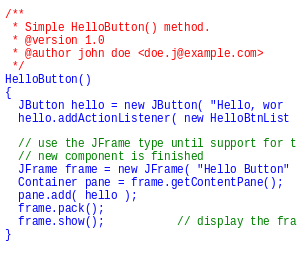
\includegraphics[scale=0.6]{figure1}
\caption{Popis obrázku.}\label{figure1}\end{center}\end{figure}

Pellentesque id sem sed nulla vehicula pellentesque. Vestibulum tincidunt faucibus tortor, et feugiat libero sagittis eget. Maecenas ultrices justo venenatis lectus malesuada gravida. Quisque commodo auctor sem, ut congue dolor ullamcorper sit amet. Sed eu dolor purus. Aliquam blandit, magna sed gravida ultrices, nibh mi porttitor erat, sed scelerisque enim magna nec risus. Mauris vestibulum arcu vel enim rhoncus eleifend. Sed nec interdum sapien. Pellentesque tincidunt condimentum consectetur. Maecenas posuere nunc in lacus consectetur sed posuere felis tristique. Vivamus diam lorem, commodo eget aliquet sed, volutpat sit amet nisi. Morbi posuere leo sit amet odio dignissim hendrerit. Praesent eget urna odio, non hendrerit neque. Suspendisse eget massa metus, in vestibulum est. Donec ac elit vitae ante auctor laoreet. Donec purus lorem, bibendum vel euismod ac, semper quis lacus~\cite{3}.

\begin{figure}[H]\begin{center}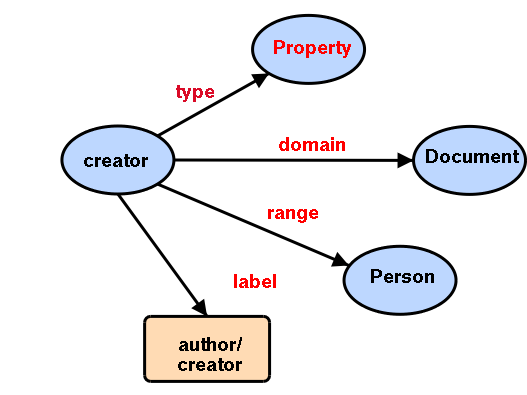
\includegraphics[scale=0.6]{figure2}
\caption{Popis obrázku; prevzaté z~\cite{3}.}\label{pic1}\end{center}
\end{figure}



%%
%% design
%%
\newpage

\section{Návrh, špecifikácia požiadaviek a pod.}
Aenean consequat, sapien a posuere tincidunt, massa purus egestas nisl, sed sollicitudin neque mi vel augue. Sed condimentum nibh ut metus condimentum ornare. Maecenas ultrices tempor condimentum. Etiam nec lorem leo, id consequat tellus. Etiam id mattis massa. Phasellus commodo, lacus in viverra lacinia, quam leo ultricies tellus, condimentum vehicula dui nisl a magna. In mi felis, malesuada eget tincidunt eget, rutrum ac lacus. In a nisl tellus. Mauris hendrerit egestas odio ac consequat. Curabitur aliquam convallis nibh sed blandit. Ut et viverra felis. Sed varius quam non mauris facilisis tincidunt. Quisque et libero eros, sed hendrerit sapien. Aliquam nec faucibus neque. Integer dictum arcu sed risus scelerisque fermentum. Pellentesque vitae ipsum lorem, sed lacinia ligula~\cite{4}.

\begin{figure}\begin{center}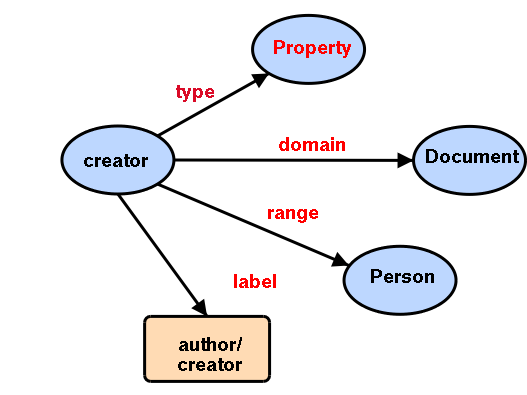
\includegraphics[scale=0.55]{figure2}
\caption{Popis schémy.}\label{figure2}
\end{center}\end{figure}

Etiam nec lorem leo, id consequat tellus. Etiam id mattis massa. Phasellus commodo, lacus in viverra lacinia, quam leo ultricies tellus, condimentum vehicula dui nisl a magna. In mi felis, malesuada eget tincidunt eget, rutrum ac lacus. In a nisl tellus. Mauris hendrerit egestas odio ac consequat. Etiam nec lorem leo, id consequat tellus. Etiam id mattis massa. Phasellus commodo, lacus in viverra lacinia, quam leo ultricies tellus, condimentum vehicula dui nisl a magna. In mi felis, malesuada eget tincidunt eget, rutrum ac lacus. In a nisl tellus. Mauris hendrerit egestas odio ac consequat. Etiam nec lorem leo, id consequat tellus. Etiam id mattis massa. Phasellus commodo, lacus in viverra lacinia, quam leo ultricies tellus, condimentum vehicula dui nisl a magna. In mi felis, malesuada eget tincidunt eget, rutrum ac lacus. In a nisl tellus. Mauris hendrerit egestas odio ac consequat.

%\lstinputlisting[float=h,language=javascript,caption={Príklad listingu zo súboru.},label={listing},frame=single,frameround=ffff,captionpos=b,basicstyle=\scriptsize]{figures/listing}

Etiam nec lorem leo, id consequat tellus. Etiam id mattis massa. Phasellus commodo, lacus in viverra lacinia, quam leo ultricies tellus, condimentum vehicula dui nisl a magna. In mi felis, malesuada eget tincidunt eget, rutrum ac lacus. In a nisl tellus. Mauris hendrerit egestas odio ac consequat. Etiam nec lorem leo, id consequat tellus. Etiam id mattis massa. Phasellus commodo, lacus in viverra lacinia, quam leo ultricies tellus, condimentum vehicula dui nisl a magna. In mi felis, malesuada eget tincidunt eget, rutrum ac lacus. In a nisl tellus. Mauris hendrerit egestas odio ac consequat. Etiam nec lorem leo, id consequat tellus. Etiam id mattis massa. Phasellus commodo, lacus in viverra lacinia, quam leo ultricies tellus, condimentum vehicula dui nisl a magna. In mi felis, malesuada eget tincidunt eget, rutrum ac lacus. In a nisl tellus. Mauris hendrerit egestas odio ac consequat.


%%
%% test
%%
\newpage

\section{Testovanie}

Aenean consequat, sapien a posuere tincidunt, massa purus egestas nisl, sed sollicitudin neque mi vel augue. Sed condimentum nibh ut metus condimentum ornare. Maecenas ultrices tempor condimentum. Etiam nec lorem leo, id consequat tellus. Etiam id mattis massa. Phasellus commodo, lacus in viverra lacinia, quam leo ultricies tellus, condimentum vehicula dui nisl a magna. In mi felis, malesuada eget tincidunt eget, rutrum ac lacus. In a nisl tellus. Mauris hendrerit egestas odio ac consequat. Curabitur aliquam convallis nibh sed blandit. Ut et viverra felis. Sed varius quam non mauris facilisis tincidunt. Quisque et libero eros, sed hendrerit sapien. Aliquam nec faucibus neque. Integer dictum arcu sed risus scelerisque fermentum. Pellentesque vitae ipsum lorem, sed lacinia ligula.

%\lstinputlisting[float=h,language=javascript,caption={Príklad listingu zo súboru.},label={listing},frame=single,frameround=ffff,captionpos=b,basicstyle=\scriptsize]{figures/listing}

\subsection{Podnadpis}\label{sub23}
Aenean consequat, sapien a posuere tincidunt, massa purus egestas nisl, sed sollicitudin neque mi vel augue. Sed condimentum nibh ut metus condimentum ornare. Maecenas ultrices tempor condimentum. Etiam nec lorem leo, id consequat tellus. Etiam id mattis massa. Phasellus commodo, lacus in viverra lacinia, quam leo ultricies tellus, condimentum vehicula dui nisl a magna. In mi felis, malesuada eget tincidunt eget, rutrum ac lacus. In a nisl tellus. Mauris hendrerit egestas odio ac consequat. Curabitur aliquam convallis nibh sed blandit. Ut et viverra felis. Sed varius quam non mauris facilisis tincidunt. Quisque et libero eros, sed hendrerit sapien. Aliquam nec faucibus neque. Integer dictum arcu sed risus scelerisque fermentum. Pellentesque vitae ipsum lorem, sed lacinia ligula~\cite{5}.

\subsubsection{Nizsi podnadpis}
Aenean consequat, sapien a posuere tincidunt, massa purus egestas nisl, sed sollicitudin neque mi vel augue. Sed condimentum nibh ut metus condimentum ornare. Maecenas ultrices tempor condimentum. Etiam nec lorem leo, id consequat tellus. Etiam id mattis massa. Phasellus commodo, lacus in viverra lacinia, quam leo ultricies tellus, condimentum vehicula dui nisl a magna. In mi felis, malesuada eget tincidunt eget, rutrum ac lacus. In a nisl tellus. Mauris hendrerit egestas odio ac consequat. Curabitur aliquam convallis nibh sed blandit. Ut et viverra felis. Sed varius quam non mauris facilisis tincidunt. Quisque et libero\footnote{\url{http://example.com}} eros, sed hendrerit sapien. Aliquam nec faucibus neque. Integer dictum arcu sed risus scelerisque fermentum. Pellentesque vitae ipsum lorem, sed lacinia ligula.

Aenean consequat, sapien a posuere tincidunt, massa purus egestas nisl, sed sollicitudin neque mi vel augue. Sed condimentum nibh ut metus condimentum ornare. Maecenas ultrices tempor condimentum. Etiam nec lorem leo, id consequat tellus. Etiam id mattis massa. Phasellus commodo, lacus in viverra lacinia, quam leo ultricies tellus, condimentum vehicula dui nisl a magna. In mi felis, malesuada eget tincidunt eget, rutrum ac lacus. In a nisl tellus. Mauris hendrerit egestas odio ac consequat. Curabitur aliquam convallis nibh sed blandit. Ut et viverra felis. Sed varius quam non mauris facilisis tincidunt. Quisque et libero eros, sed hendrerit sapien. Aliquam nec faucibus neque. Integer dictum arcu sed risus scelerisque fermentum. Pellentesque vitae ipsum lorem, sed lacinia ligula.


%%
%% Conclusion
%%
\newpage

\section{Zhodnotenie}

Pellentesque id sem sed nulla vehicula pellentesque. Vestibulum tincidunt faucibus tortor, et feugiat libero sagittis eget. Maecenas ultrices justo venenatis lectus malesuada gravida. Quisque commodo auctor sem, ut congue dolor ullamcorper sit amet. Sed eu dolor purus. Aliquam blandit, magna sed gravida ultrices, nibh mi porttitor erat, sed scelerisque enim magna nec risus. Mauris vestibulum arcu vel enim rhoncus eleifend. Sed nec interdum sapien. Pellentesque tincidunt condimentum consectetur. Maecenas posuere nunc in lacus consectetur sed posuere felis tristique. Vivamus diam lorem, commodo eget aliquet sed, volutpat sit amet nisi. Morbi posuere leo sit amet odio dignissim hendrerit. Praesent eget urna odio, non hendrerit neque. Suspendisse eget massa metus, in vestibulum est. Donec ac elit vitae ante auctor laoreet. Donec purus lorem, bibendum vel euismod ac, semper quis lacus.

Pellentesque id sem sed nulla vehicula pellentesque. Vestibulum tincidunt faucibus tortor, et feugiat libero sagittis eget. Maecenas ultrices justo venenatis lectus malesuada gravida. Quisque commodo auctor sem, ut congue dolor ullamcorper sit amet. Sed eu dolor purus. Aliquam blandit, magna sed gravida ultrices, nibh mi porttitor erat, sed scelerisque enim magna nec risus. Mauris vestibulum arcu vel enim rhoncus eleifend. Sed nec interdum sapien. Pellentesque tincidunt condimentum consectetur. Maecenas posuere nunc in lacus consectetur sed posuere felis tristique. Vivamus diam lorem, commodo eget aliquet sed, volutpat sit amet nisi. Morbi posuere leo sit amet odio dignissim hendrerit. Praesent eget urna odio, non hendrerit neque. Suspendisse eget massa metus, in vestibulum est. Donec ac elit vitae ante auctor laoreet. Donec purus lorem, bibendum vel euismod ac, semper quis lacus.

\subsection{Možné vylepšenia}
Pellentesque id sem sed nulla vehicula pellentesque. Vestibulum tincidunt faucibus tortor, et feugiat libero sagittis eget. Maecenas ultrices justo venenatis lectus malesuada gravida. Quisque commodo auctor sem, ut congue dolor ullamcorper sit amet. Sed eu dolor purus. Aliquam blandit, magna sed gravida ultrices, nibh mi porttitor erat, sed scelerisque enim magna nec risus. Mauris vestibulum arcu vel enim rhoncus eleifend. Sed nec interdum sapien~\cite{4}.

Pellentesque tincidunt condimentum consectetur. Maecenas posuere nunc in lacus consectetur sed posuere felis tristique. Vivamus diam lorem, commodo eget aliquet sed, volutpat sit amet nisi. Morbi posuere leo sit amet odio dignissim hendrerit. Praesent eget urna odio, non hendrerit neque. Suspendisse eget massa metus, in vestibulum est. Donec ac elit vitae ante auctor laoreet. Donec purus lorem, bibendum vel euismod ac, semper quis lacus.


%%
%% References
%%
\newpage
\addcontentsline{toc}{section}{\refname}
\bibliographystyle{apalike}
\begin{flushleft}
\bibliography{references}
\end{flushleft}

%%
%% Appendix
%%
\ifthenelse {\boolean{bachelor}}
{
}
{
	\ifthenelse {\boolean{english}}
	{
		\renewcommand{\appendixname}{Appendix}
		\renewcommand{\appendixtocname}{Appendix}
	}
	{
		\renewcommand{\appendixname}{Príloha}
		\renewcommand{\appendixtocname}{Prílohy}
	}
	\pagenumbering{bychapter}
}
\appendix
\newpage
\thispagestyle{plain}

\section{Technická dokumentácia}\label{technical_documentation}

Lorem ipsum dolor sit amet, consectetur adipiscing elit. Duis interdum pretium orci, at cursus nisi cursus at. Pellentesque ultricies eros fermentum massa cursus fringilla. Vestibulum aliquam, magna a adipiscing elementum, tortor neque lobortis metus, sit amet consectetur ipsum leo quis dui. Vestibulum sit amet nisi sit amet felis tempor feugiat. Morbi sagittis luctus risus molestie mattis. Cras turpis mauris, lacinia a eleifend in, semper a augue. Aenean ultrices rhoncus metus ut auctor. Pellentesque fermentum justo eget erat commodo vel mollis augue semper. Nunc tempor augue nulla, pellentesque posuere orci.

Integer lorem sapien, sollicitudin ac aliquet in, posuere et sapien. Nam non vulputate ipsum. Suspendisse quis ante in arcu sagittis auctor sed nec arcu. Cras condimentum massa eu arcu hendrerit ac iaculis nibh euismod. Vivamus non felis consectetur sem pretium ornare. Etiam ipsum ante, laoreet rhoncus ullamcorper nec, cursus non mi. Nunc lacinia lectus id sem consequat varius. Praesent pellentesque, leo nec vulputate egestas, dui arcu consequat nisi, et convallis augue elit in lacus. Nulla luctus faucibus lacinia. Pellentesque interdum ligula non mauris dignissim molestie.

Pellentesque id sem sed nulla vehicula pellentesque. Vestibulum tincidunt faucibus tortor, et feugiat libero sagittis eget. Maecenas ultrices justo venenatis lectus malesuada gravida. Quisque commodo auctor sem, ut congue dolor ullamcorper sit amet. Sed eu dolor purus. Aliquam blandit, magna sed gravida ultrices, nibh mi porttitor erat, sed scelerisque enim magna nec risus. Mauris vestibulum arcu vel enim rhoncus eleifend. Sed nec interdum sapien. Pellentesque tincidunt condimentum consectetur. Maecenas posuere nunc in lacus consectetur sed posuere felis tristique. Vivamus diam lorem, commodo eget aliquet sed, volutpat sit amet nisi. Morbi posuere leo sit amet odio dignissim hendrerit. Praesent eget urna odio, non hendrerit neque. Suspendisse eget massa metus, in vestibulum est. Donec ac elit vitae ante auctor laoreet. Donec purus lorem, bibendum vel euismod ac, semper quis lacus.

Cum sociis natoque penatibus et magnis dis parturient montes, nascetur ridiculus mus. Integer turpis lacus, convallis porta aliquam eu, luctus in orci. Duis tincidunt condimentum augue in laoreet. Vivamus tempus iaculis ligula, dictum dignissim nibh elementum at. Donec quis risus quis sem blandit auctor. Integer eu tellus nisi, et fringilla magna. Praesent vulputate placerat pretium. Etiam vitae ornare est.

\newpage
\section{Používateľská dokumentácia}
Integer lorem sapien, sollicitudin ac aliquet in, posuere et sapien. Nam non vulputate ipsum. Suspendisse quis ante in arcu sagittis auctor sed nec arcu.

\subsection{Inštalačná príručka}\label{install_guide}

\subsubsection{Nadpis1}
Integer lorem sapien, sollicitudin ac aliquet in, posuere et sapien. Nam non vulputate ipsum. Suspendisse quis ante in arcu sagittis auctor sed nec arcu. Cras condimentum massa eu arcu hendrerit ac iaculis nibh euismod. Vivamus non felis consectetur sem pretium ornare. Etiam ipsum ante, laoreet rhoncus ullamcorper nec, cursus non mi. Nunc lacinia lectus id sem consequat varius. Praesent pellentesque, leo nec vulputate egestas, dui arcu consequat nisi, et convallis augue elit in lacus. Nulla luctus faucibus lacinia. Pellentesque interdum ligula non mauris dignissim molestie.

\subsubsection{Nadpis2}
Integer lorem sapien, sollicitudin ac aliquet in, posuere et sapien. Nam non vulputate ipsum. Suspendisse quis ante in arcu sagittis auctor sed nec arcu. Cras condimentum massa eu arcu hendrerit ac iaculis nibh euismod. Vivamus non felis consectetur sem pretium ornare. Etiam ipsum ante, laoreet rhoncus ullamcorper nec, cursus non mi. Nunc lacinia lectus id sem consequat varius. Praesent pellentesque, leo nec vulputate egestas, dui arcu consequat nisi, et convallis augue elit in lacus. Nulla luctus faucibus lacinia. Pellentesque interdum ligula non mauris dignissim molestie.

\newpage
\subsection{Používateľská príručka}
Integer lorem sapien, sollicitudin ac aliquet in, posuere et sapien. Nam non vulputate ipsum. Suspendisse quis ante in arcu sagittis auctor sed nec arcu.

\subsubsection{Nadpis3}
Integer lorem sapien, sollicitudin ac aliquet in, posuere et sapien. Nam non vulputate ipsum. Suspendisse quis ante in arcu sagittis auctor sed nec arcu. Cras condimentum massa eu arcu hendrerit ac iaculis nibh euismod. Vivamus non felis consectetur sem pretium ornare. Etiam ipsum ante, laoreet rhoncus ullamcorper nec, cursus non mi. Nunc lacinia lectus id sem consequat varius. Praesent pellentesque, leo nec vulputate egestas, dui arcu consequat nisi, et convallis augue elit in lacus. Nulla luctus faucibus lacinia. Pellentesque interdum ligula non mauris dignissim molestie.

\newpage
\section{Elektronické médium}

K dokumentu priložené elektronické médium má nasledovnú štruktúru:
\begin{my_itemize}

\emptyitem /doc
	\begin{my_itemize}
	\myitem bakalárska práca spolu s anotáciami v slovenskom a anglickom jazyku
	\end{my_itemize}

\emptyitem /doc/bibtex
	\begin{my_itemize}
	\myitem súbor s referenciami vo formáte BibTeX
	\end{my_itemize}

\emptyitem /doc/latex
	\begin{my_itemize}
	\myitem súbory dokumentácie vo formáte Latex
	\end{my_itemize}

\emptyitem /doc/resources
	\begin{my_itemize}
	\myitem dostupné použité zdroje
	\end{my_itemize}

\emptyitem /source
	\begin{my_itemize}
	\myitem zdrojové kódy samotnej implementovanej aplikácie
	\end{my_itemize}

\emptyitem readme.txt
	\begin{my_itemize}
    \myitem popis obsahu média v slovenskom a~anglickom jazyku
	\end{my_itemize}
\end{my_itemize}


\end{document}

%%%%%%%%%%%%%%%%%%%%%%%%%%%%%%%%%%%%%%%%%%%%%%%%%%%%%%%%%%%%%%%%%%%%%%%%%%%%%%%%%%%%%%%%

%%
%% !!!! set your own details
%%
\begin{comment}
[x] [Autor Dokumentu], [Nazov Stranky], [URL], [Datum Navstevy]
\end{comment}
